%!TEX root = book.tex
\chapter{โจทย์ปริศนา Final Round}

\newpage
\setSpacing{1.5}
\section{Question 1}

มีของเล่นทั้งสิ้น 2019 ชนิด ชนิดละหลายชิ้น ต้องการนำของเล่นดังกล่าวไปแจกให้เด็กเป็นจำนวนคนมากที่สุดโดยที่สอดคล้องกับเงื่อนไขว่า
\begin{itemize}[topsep=0pc,itemsep=0pc]
\item เด็กแต่ละคนจะต้องได้ของขวัญอย่างน้อย 1 ชิ้น และ\uline{ชนิดละไม่เกิน 1 ชิ้น}
\item สำหรับเด็ก $x$ และ $y$ สองคนใด ๆ จะต้องพบว่าเงื่อนไขย่อยต่อไปนี้จะเป็นจริง 1 ข้อ
    \begin{itemize}[topsep=0pc,itemsep=0pc]
        \item  $x$ มีของเล่นทุกชนิดที่ $y$ มี แต่มีของเล่นของ $x$ บางชนิดที่ $y$ ไม่มี
        \item  $y$ มีของเล่นทุกชนิดที่ $x$ มี แต่มีของเล่นของ $y$ บางชนิดที่ $x$ ไม่มี
        \item  $x$ และ $y$ ไม่ครอบครองของเล่นชนิดใดร่วมกันเลย
    \end{itemize}
\end{itemize}
อยากทราบว่าเราจะต้องเตรียมของเล่น\uline{อย่างน้อย}ที่สุดกี่ชิ้น และ\uline{อย่างมาก}ที่สุดกี่ชิ้น?


\setSpacing{1.5}
\section{Question 2}

มีการ์ดไพ่ทั้งสิ้น 6 ใบ แต่ละใบเขียนหมายเลข 1 ถึง 6 หมายเลขละหนึ่งใบพอดี \;
ไพ่ทั้ง 6 ใบนี้ถูกนำมาวางเรียงกันเป็นแถวอยู่แถวหนึ่ง \;
เราจะกล่าวว่าไพ่ใบหนึ่ง ({\hrsp}ชึ่งเขียนหมายเลข $i${\hrsp}) \uline{อยู่ในตำแหน่งที่ถูกต้อง}ก็ต่อเมื่อไพ่ใบดังกล่าวอยู่ในตำแหน่งที่ $i$ โดยเริ่มนับจากใบซ้ายสุดเป็นไพ่ใบแรก

\begin{itemize}[topsep=0pc,itemsep=0pc]
\item  ในตอนแรกเริ่ม ไม่มีไพ่ใบใดที่อยู่ในตำแหน่งที่ถูกต้องเลย
    \begin{center}
        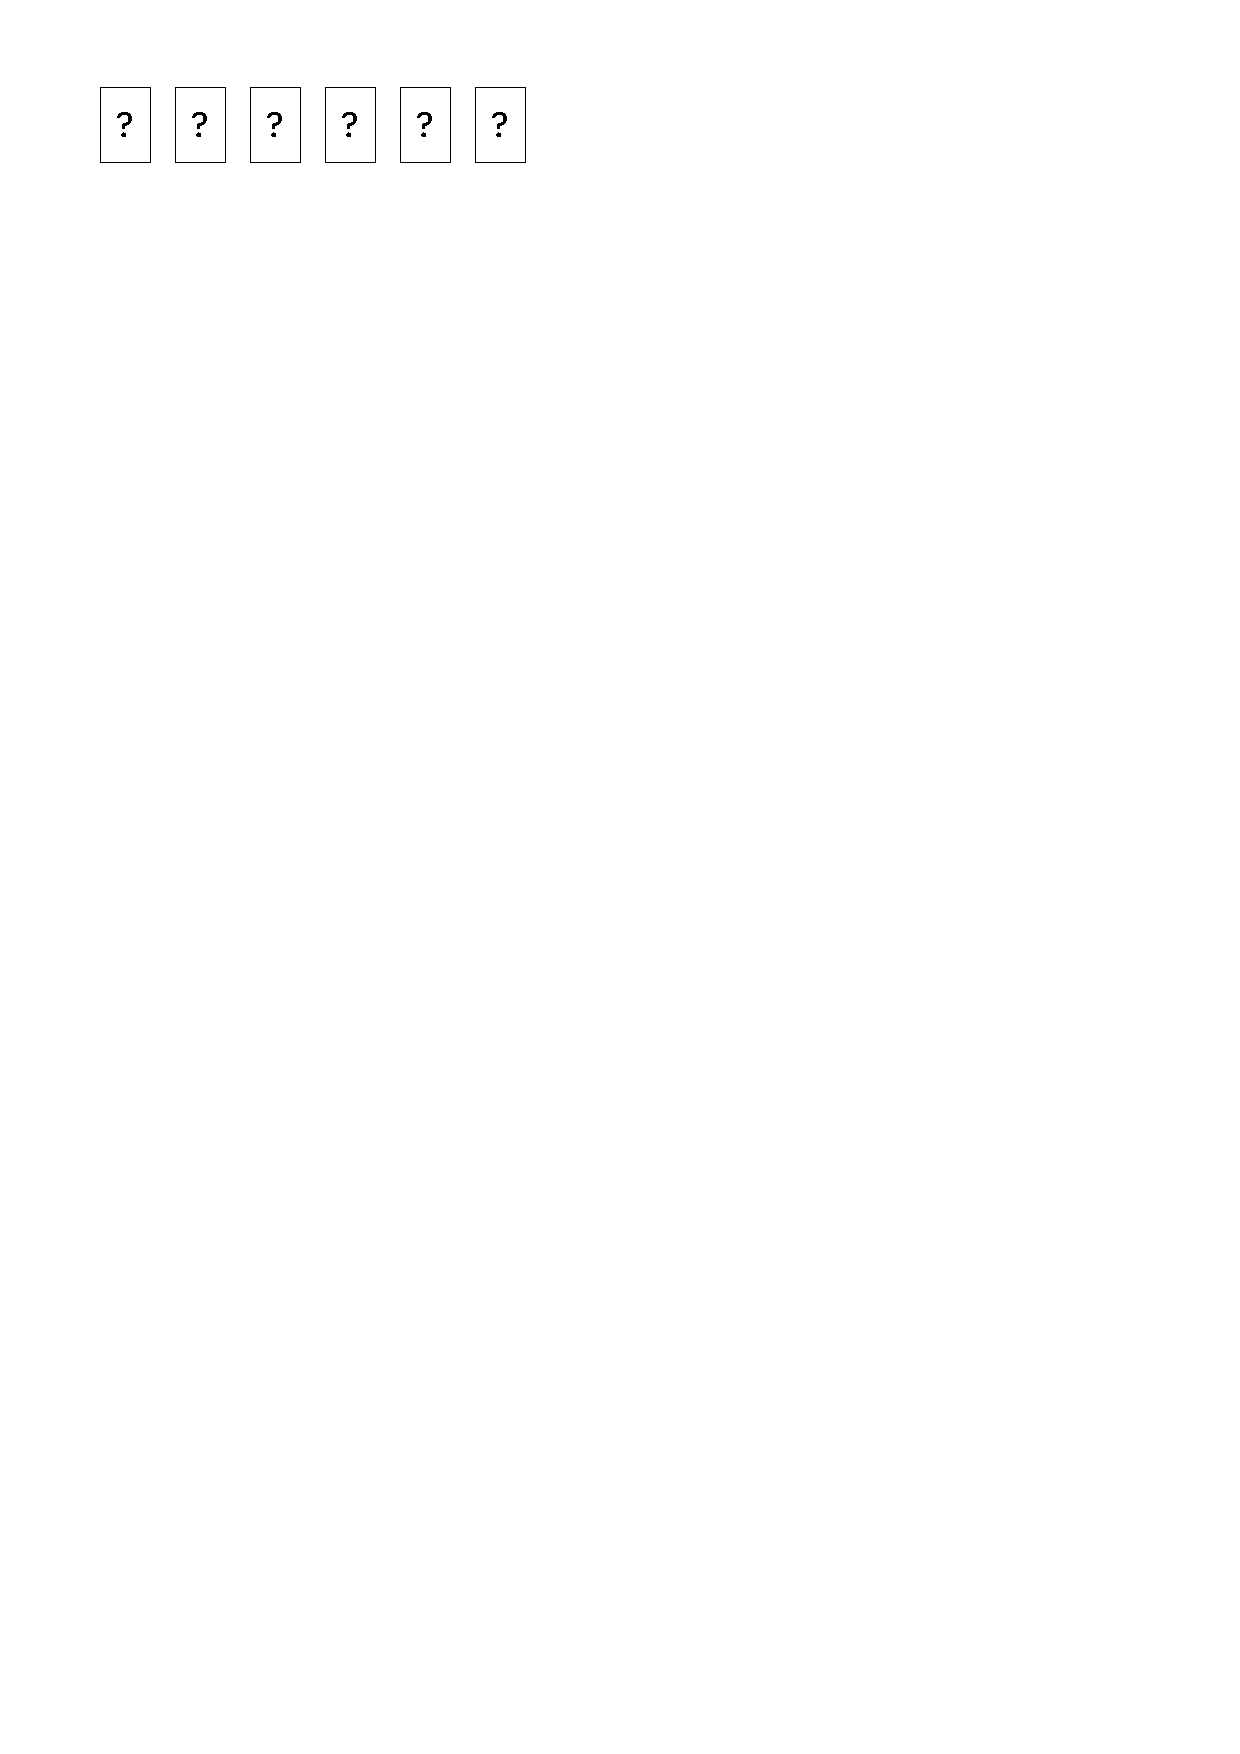
\includegraphics[page=1]{figures/puzzle.pdf}
    \end{center}
\item  จากนั้นเราเลือกสลับไพ่คู่หนึ่งที่อยู่ติดกัน \; พบว่ามีไพ่ 1 ใบอยู่ในตำแหน่งที่ถูกต้อง
\item  จากนั้นสลับไพ่อีกคู่หนึ่งที่อยู่ติดกัน (ซึ่งเป็นคนละคู่กับรอบที่แล้ว) \; พบว่ามีไพ่ 2 ใบอยู่ในตำแหน่งที่ถูกต้อง
\item  จากนั้นสลับไพ่อีกคู่หนึ่งที่อยู่ติดกัน (ซึ่งเป็นคนละคู่กับรอบที่แล้ว) \; พบว่ามีไพ่ 1 ใบอยู่ในตำแหน่งที่ถูกต้อง
\item  จากนั้นสลับไพ่อีกคู่หนึ่งที่อยู่ติดกัน (ซึ่งเป็นคนละคู่กับรอบที่แล้ว) \; พบว่ามีไพ่ 1 ใบอยู่ในตำแหน่งที่ถูกต้อง
\item  จากนั้นสลับไพ่อีกคู่หนึ่งที่อยู่ติดกัน (ซึ่งเป็นคนละคู่กับรอบที่แล้ว) \; พบว่ามีไพ่ 2 ใบอยู่ในตำแหน่งที่ถูกต้อง
\item  จากนั้นสลับไพ่อีกคู่หนึ่งที่อยู่ติดกัน (ซึ่งเป็นคนละคู่กับรอบที่แล้ว) \; พบว่ามีไพ่ 3 ใบอยู่ในตำแหน่งที่ถูกต้อง
\item  จากนั้นสลับไพ่อีกคู่หนึ่งที่อยู่ติดกัน (ซึ่งเป็นคนละคู่กับรอบที่แล้ว) \; พบว่ามีไพ่ 4 ใบอยู่ในตำแหน่งที่ถูกต้อง
\item  จากนั้นสลับไพ่อีกคู่หนึ่งที่อยู่ติดกัน (ซึ่งเป็นคนละคู่กับรอบที่แล้ว) \; พบว่าไพ่ทุกใบอยู่ในตำแหน่งที่ถูกต้อง
    \begin{center}
        \includegraphics[page=2]{figures/puzzle.pdf}
    \end{center}
\end{itemize}
อยากทราบว่าไพ่ทั้ง 6 ใบในตอนแรกเริ่มคือหมายเลขใดบ้างตามลำดับ?


\newpage
\setSpacing{1.5}
\section{Question 3}

จงเติมจำนวนเต็ม 1 ถึง 15 ลงในพิระมิดต่อไปนี้ ช่องละ 1 จำนวนโดยไม่ใช้จำนวนซ้ำกัน โดยที่สอดคล้องกับเงื่อนไขดังต่อไปนี้

\begin{minipage}{0.4\linewidth}
    \begin{itemize}[topsep=0pc,itemsep=0pc,leftmargin=0pc]
        \item สำหรับแต่ละพิระมิดย่อย \raisebox{-6pt}{\includegraphics[page=4]{figures/puzzle.pdf}} ที่ปรากฏในพิระมิดใหญ่ด้านล่าง จะพบว่าจำนวนในช่อง ก จะเป็นผลรวมหรือผลต่างของจำนวนในช่อง ข และ ค
        \item จำนวนในช่องต่าง ๆ จะสอดคล้องกับอสมการ \\ A < E < N, L < H < F, และ Q < J < D
    \end{itemize}
    \vspace*{4pc}
\end{minipage}
\begin{minipage}{0.525\linewidth}
    \begin{center}
        \includegraphics[page=3]{figures/puzzle.pdf}
    \end{center}    
\end{minipage}


\setSpacing{1.5}
\section{Question 4}

จงเติมจำนวนเต็ม 1 ถึง 16 ลงในตารางขนาด $4 \times 4$ ดังต่อไปนี้ ช่องละ 1 จำนวนโดยไม่ใช้จำนวนซ้ำกัน โดยกำหนดนิยามผลรวมในแนวเส้นตรงดังนี้

\medskip

\begin{minipage}{0.4\linewidth}
    \begin{itemize}[topsep=0pc,itemsep=0pc,leftmargin=0pc]
        \item  กำหนดให้ $c_1, c_2, c_3, c_4$ คือผลรวมในแนวตั้งของคอลัมน์ที่ 1, 2, 3, 4 ตามลำดับ
        \item  กำหนดให้ $r_1, r_2, r_3, r_4$ คือผลรวมในแนวนอนของแถวที่ 1, 2, 3, 4 ตามลำดับ
        \item  กำหนดให้ $d_1$ คือผลรวมแนวทแยงจากบนขวาไปล่างซ้าย 
        \item  กำหนดให้ $d_2$ คือผลรวมแนวทแยงจากบนซ้ายไปล่างขวา
    \end{itemize}
    \vspace*{1pc}
\end{minipage}
\begin{minipage}{0.525\linewidth}
    \begin{center}
        \includegraphics[page=5]{figures/puzzle.pdf}
    \end{center}    
\end{minipage}

\noindent
และการเติมจำนวนต้องสอดคล้องกับเงื่อนไขดังต่อไปนี้

\begin{itemize}[topsep=0pc,itemsep=0pc]
\item  จำนวนเต็มสองจำนวนที่อยู่ติดกัน จะต้องไม่อยู่ในช่องติดกันในตาราง ในแนวตั้งและแนวนอน
\item  ผลรวมเป็นไปตามอสมการ $c_1 < c_2 < c_3 < c_4$ และ $r_1 < r_2 < r_3 < r_4$
\item  และเซต $\{c_1, c_2, c_3, c_4, r_1, r_2, r_3, r_4, d_1, d_2\} = \{23, 27, 30, 31, 36, 37, 39, 40, 43, 48\}$
\end{itemize}


\newpage
\setSpacing{1.5}
\section{Question 5}

จงเติมเลขโดด 0 ถึง 9 ลงในตาราง Crossword ดังที่แสดงอยู่นี้ ช่องละ 1 ตัวโดยไม่ใช้เลขโดดซ้ำกัน ทำให้เกิดจำนวน 5 จำนวนเมื่ออ่านตามแนว 1–Down, 2–Across, 3–Down, 4–Across, และ 5–Across ที่สอดคล้องกับเงื่อนไขดังต่อไปนี้

\medskip

\begin{minipage}{0.5\linewidth}
    \begin{itemize}[topsep=0pc,itemsep=0pc,leftmargin=0pc]
        \item  จำนวนทั้ง 5 จำนวน ไม่ขึ้นต้นด้วยเลขโดด 0
        \item  จำนวนทั้ง 5 จำนวน เป็นจำนวนเฉพาะ
        \item  ผลรวมของจำนวนทั้ง 5 จำนวนข้างต้น ก็เป็นจำนวนเฉพาะเช่นกัน
    \end{itemize}
    \vspace*{6pc}
\end{minipage}
\begin{minipage}{0.425\linewidth}
    \begin{center}
        \includegraphics[page=6]{figures/puzzle.pdf}
    \end{center}    
\end{minipage}